\documentclass{article}
\usepackage{graphicx} % Required for inserting images
\usepackage{amsmath}
\usepackage{xeCJK}
\usepackage{amssymb}
\usepackage{indentfirst}
\usepackage{float}
\usepackage[a4paper, total={6in, 10in}]{geometry}

\title{Mathcamp 2026 Qualifying Quiz Problem 1 Solution}
\author{Applicant ID: 25107}
\date{}

\begin{document}

\maketitle

\section*{Part a)}
We claim that all players can be eliminated for all even integers $n$ except $2$ or $6$. First, we show that this is sufficient. If $n$ is of the form $4m$ with $m > 0$, we can have the following configuration:

\begin{figure}[h]
    \centering
    \vspace{-0.3cm}
    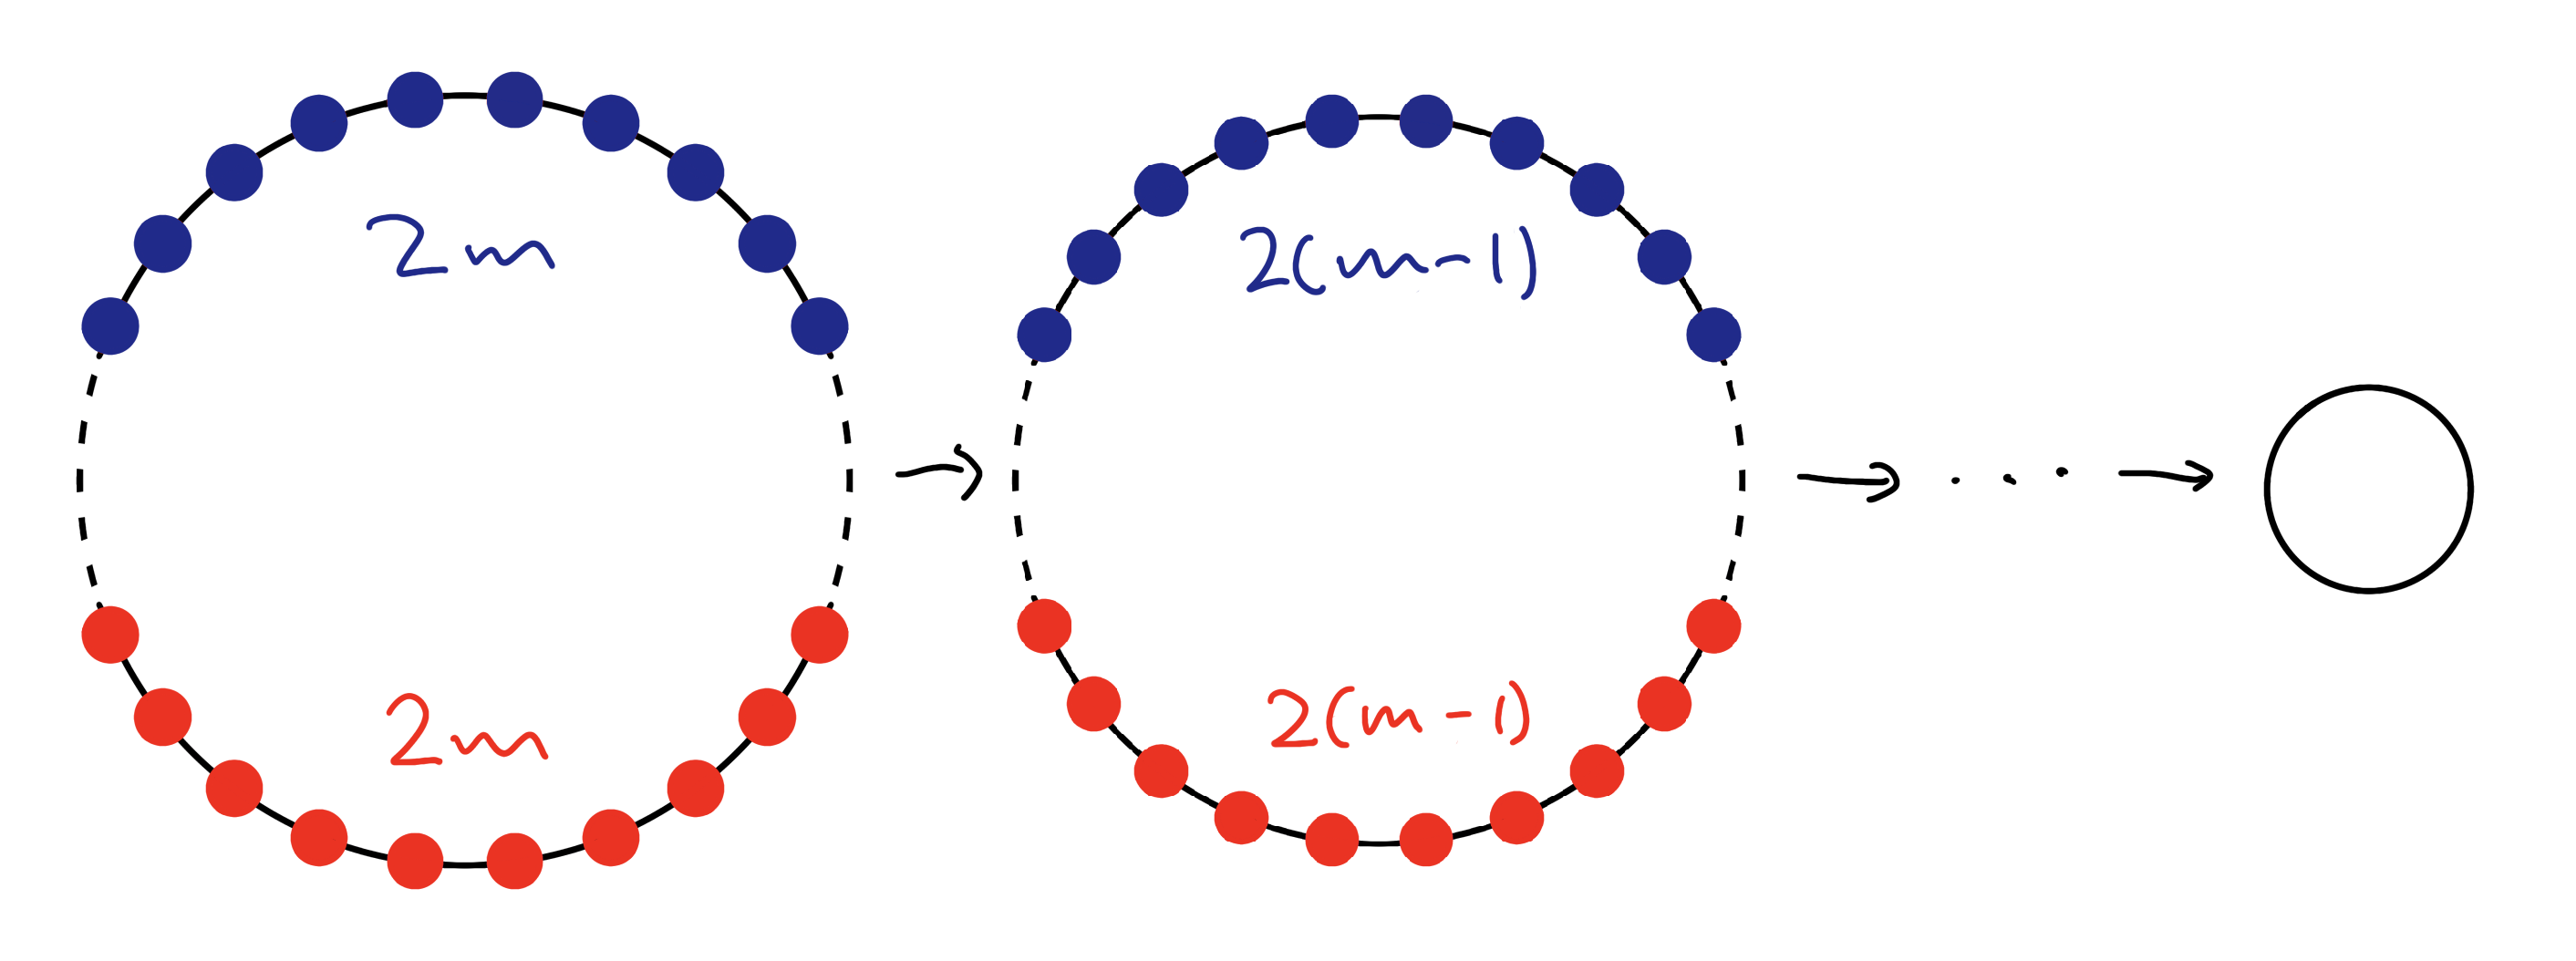
\includegraphics[width=11cm]{slow4.png}
    \vspace{-0.3cm}
\end{figure}
Here, 4 players will be eliminated each round, two of each color, until after $m$ turns there are no players left.

If instead $n$ is of the form $4m + 2$ with $m > 1$, we can have the following configuration:

\begin{figure}[h]
    \centering
    \vspace{-0.3cm}
    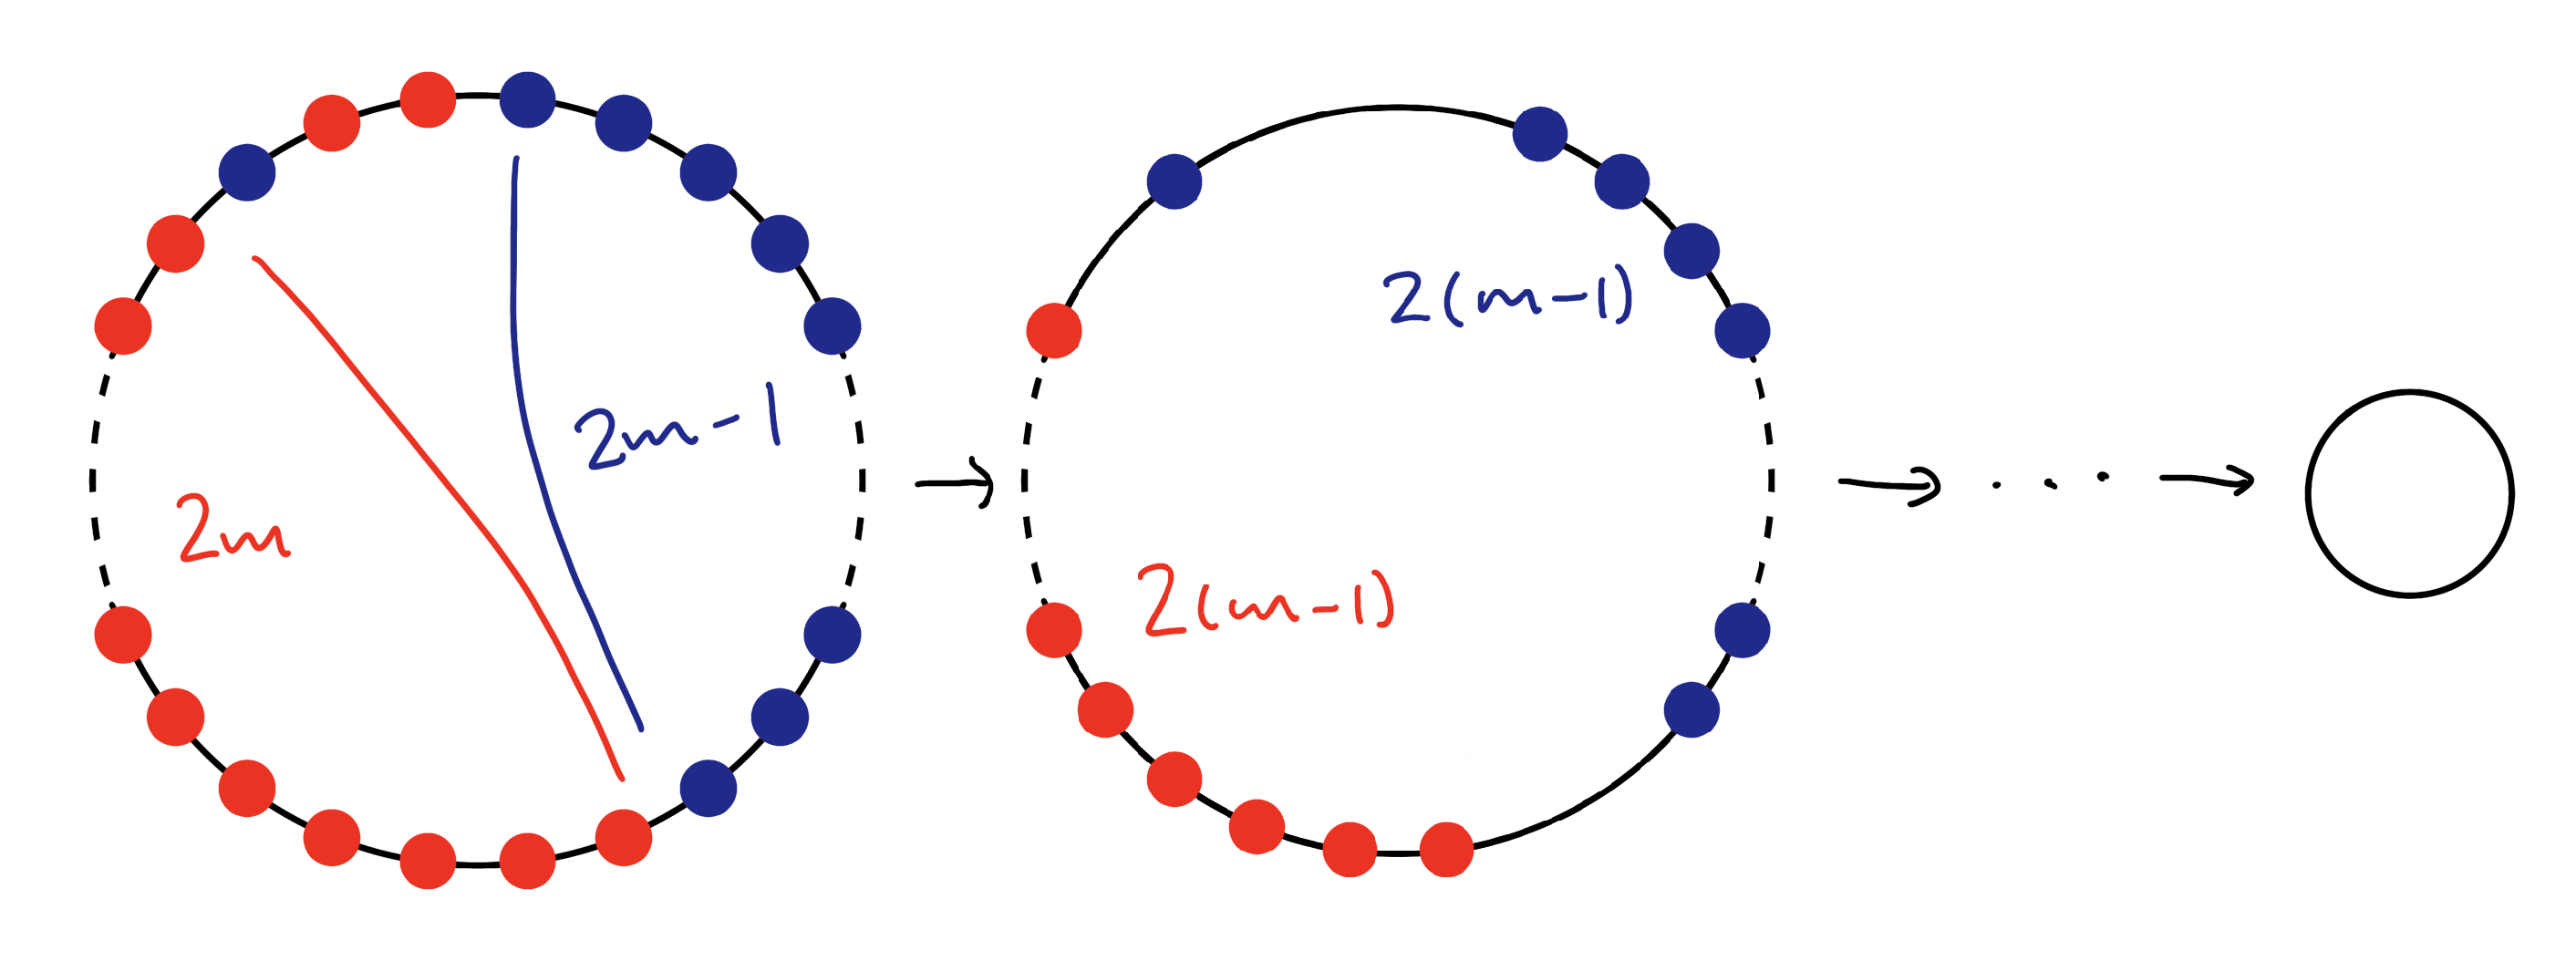
\includegraphics[width=11cm]{slow6.png}
    \vspace{-0.3cm}
\end{figure}
Here, in the first round, 6 players will be eliminated, leaving $4(m - 1)$ players exactly in the previous configuration for multiples of 4. \\

To show that our condition is necessary, we first show that $n$ must be even. Consider `blocks' of contiguous people with the same hat color. In each round, if a block contains more than one person, then we see that the two people at the ends of the block are eliminated. If a block consists of a single person, then as that person has two neighbors of the same color, they are not eliminated. Therefore, the number of eliminations each round, and therefore in total, is even. Hence $n$ is even. \\

Next, we show that $n = 2$ and $n = 6$ do not work. It is clear that when $n = 2$, no player can be eliminated as their left neighbor is the same person as their right neighbor. As we have already established that only an even number of eliminations occur each round, for $n = 6$ to be possible we must eliminate 2 players in the first round and 4 players in the next, or eliminate all players in the first round. However, to eliminate $2$ in one round, we must have two blocks containing 1 and 5 people respectively, and to eliminate $6$ people in one round we must have $3$ blocks of 2 people each which is absurd. Therefore, $n = 2$ and $n = 6$ are not possible.
\section*{Part b)}
We first consider the case when $n = 4m$ where $m > 0$. It is possible to eliminate all players in one round, as shown below:\\
\begin{figure}[h]
    \centering
    \vspace{-0.3cm}
    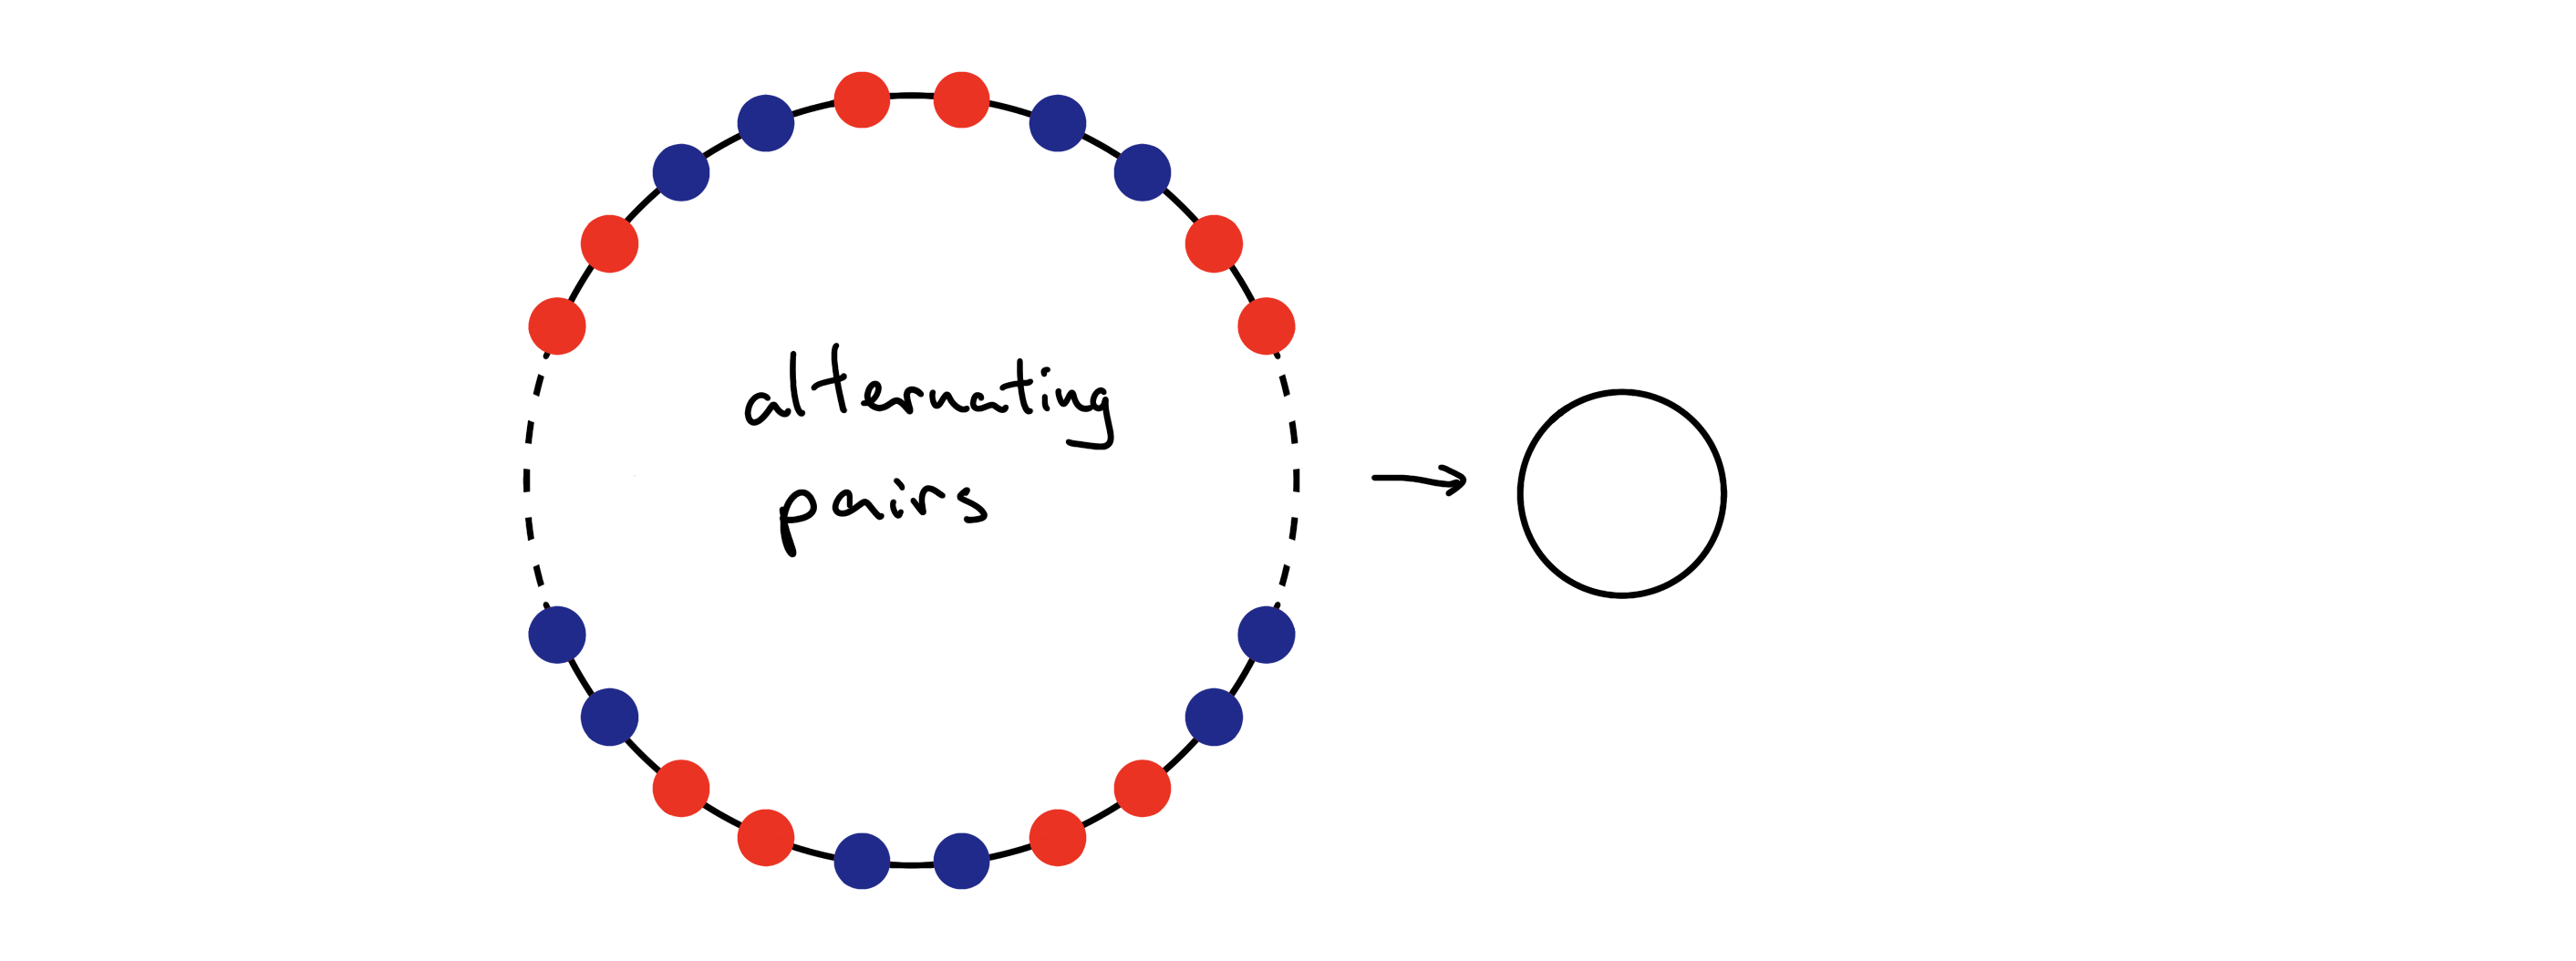
\includegraphics[width=11cm]{fast4.png}
    \vspace{-0.3cm}
\end{figure}

For the maximum number of rounds, note that there are at least $2$ blocks. As $n$ is a multiple of $4$, we cannot have both blocks consist of an odd number of people, as this would mean one block will be larger than the other, so after enough rounds there will be a single person block which cannot be eliminated. Therefore, we must have 2 blocks of $2n$ people each, with $4$ people being eliminated each round, taking a total of $m$ rounds like so:\\
\begin{figure}[h]
    \centering
    \vspace{-0.3cm}
    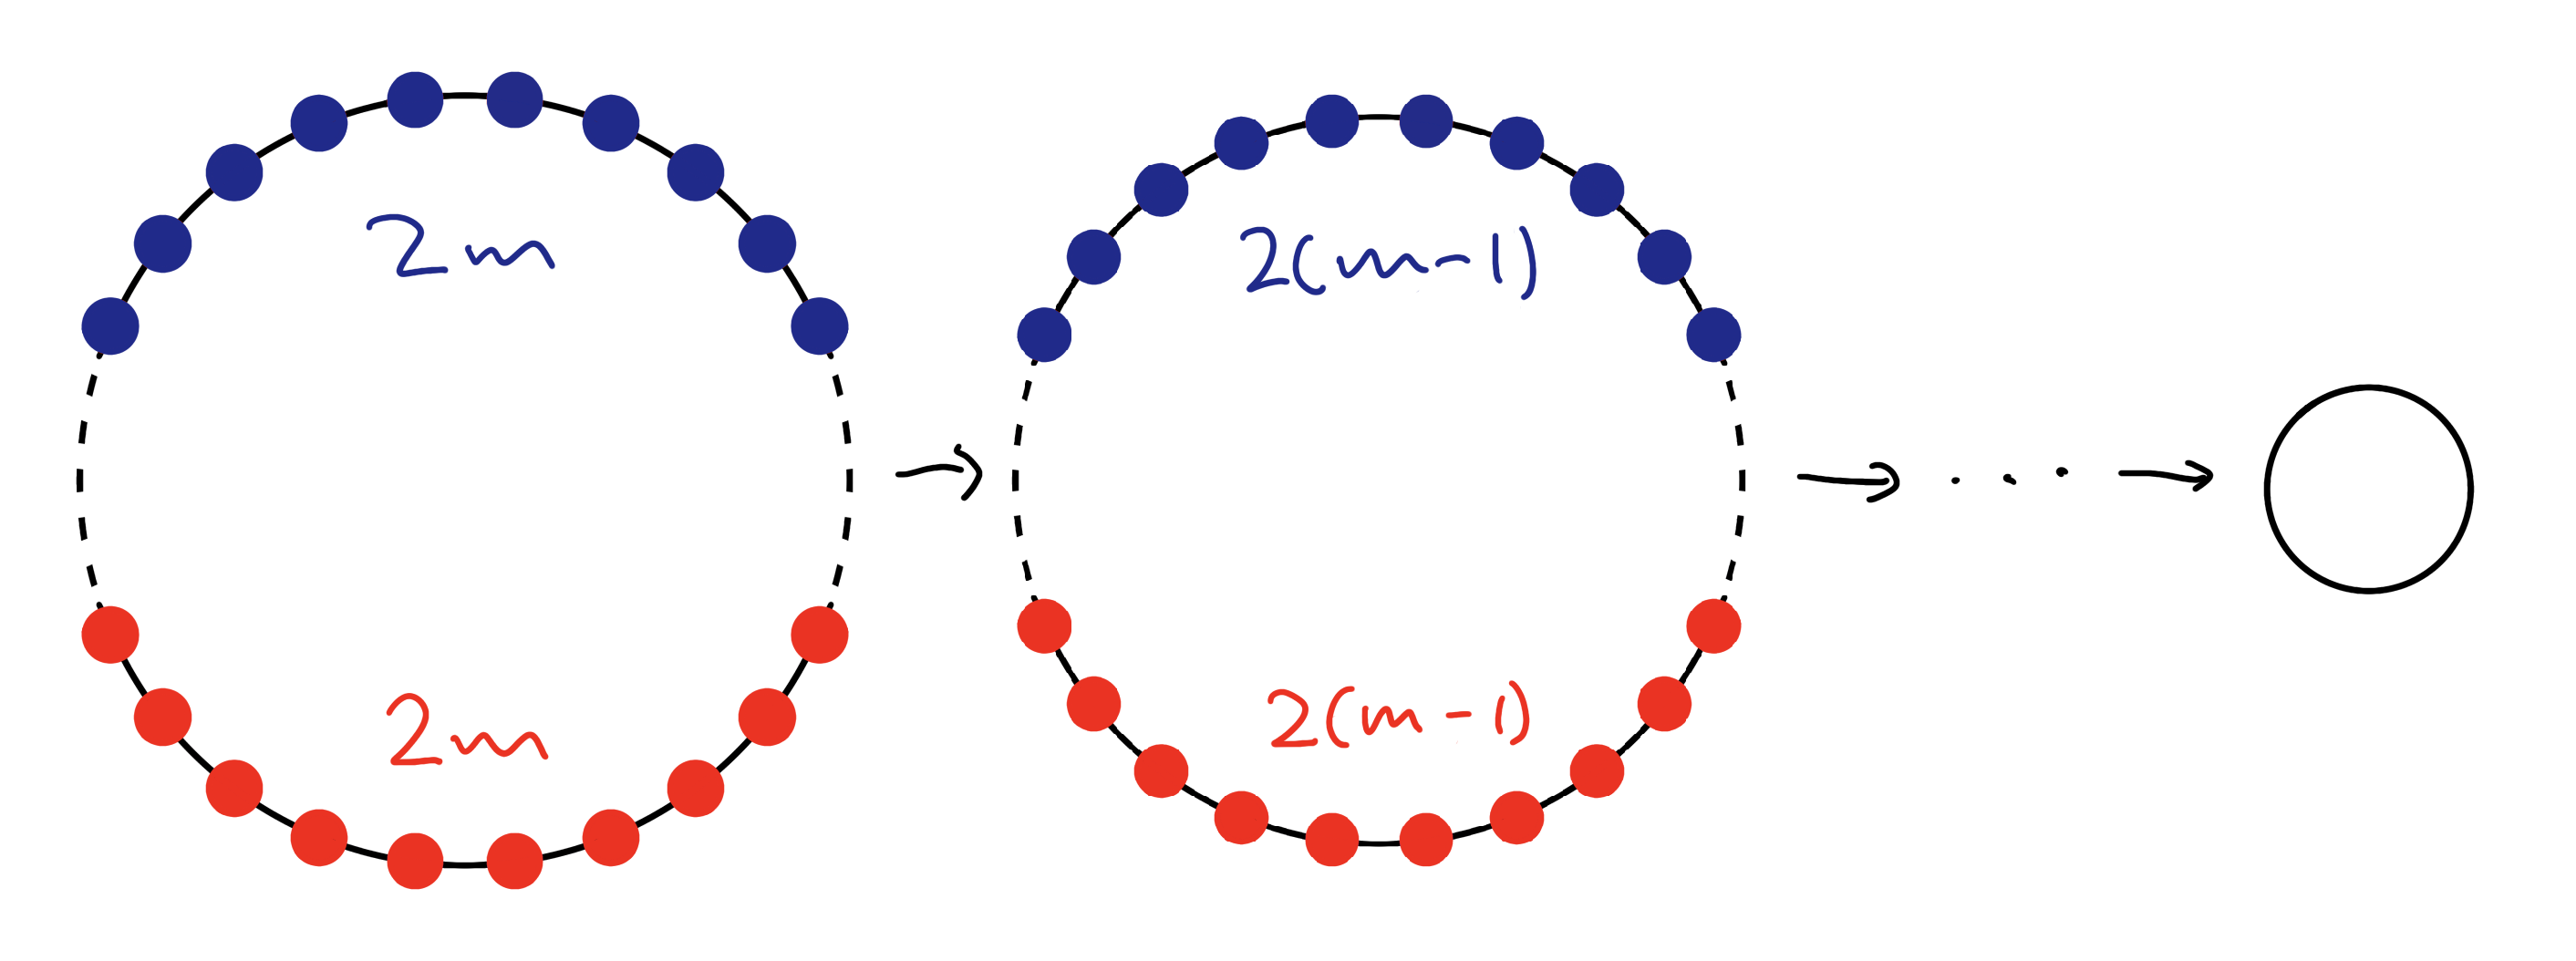
\includegraphics[width=11cm]{slow4.png}
    \vspace{-0.3cm}
\end{figure}

Now, consider when $n = 4m + 2$ where $m > 1$. It is impossible to eliminate everyone in one round as that would imply an odd number ($2m + 1$) of blocks, but it is possible in two rounds, like so:\\
\begin{figure}[h]
    \centering
    \vspace{-0.3cm}
    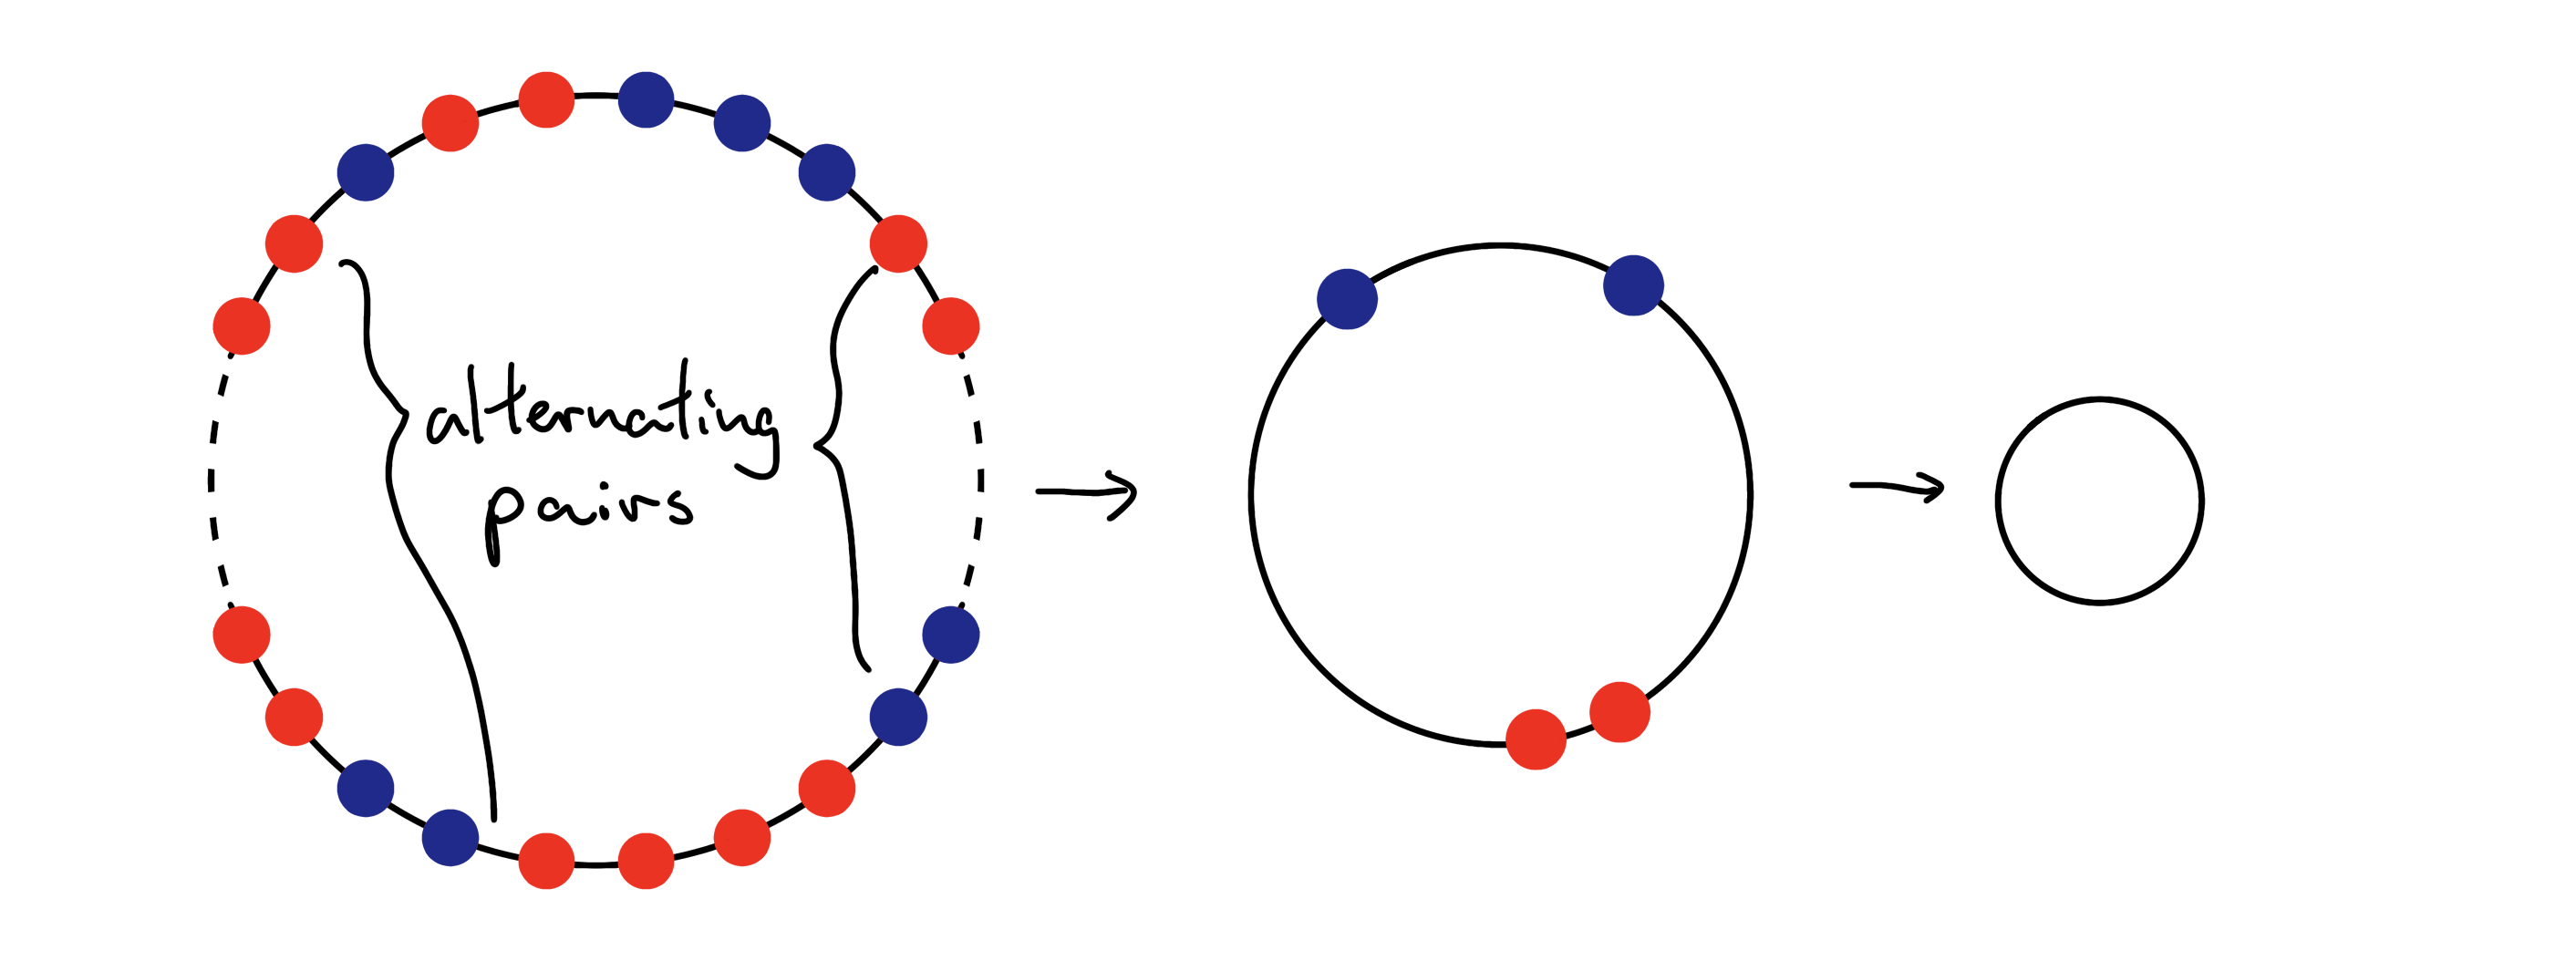
\includegraphics[width=11cm]{fast6.png}
    \vspace{-0.3cm}
\end{figure}

For the maximum number of rounds, note that we must have one round that has $4k + 2$ eliminations, following which we will have a multiple of 4, which we already have an upper bound for. Therefore, we can have the following configuration which will eliminate everyone in $m$ rounds:
\begin{figure}[H]
    \centering
    \vspace{-0.3cm}
    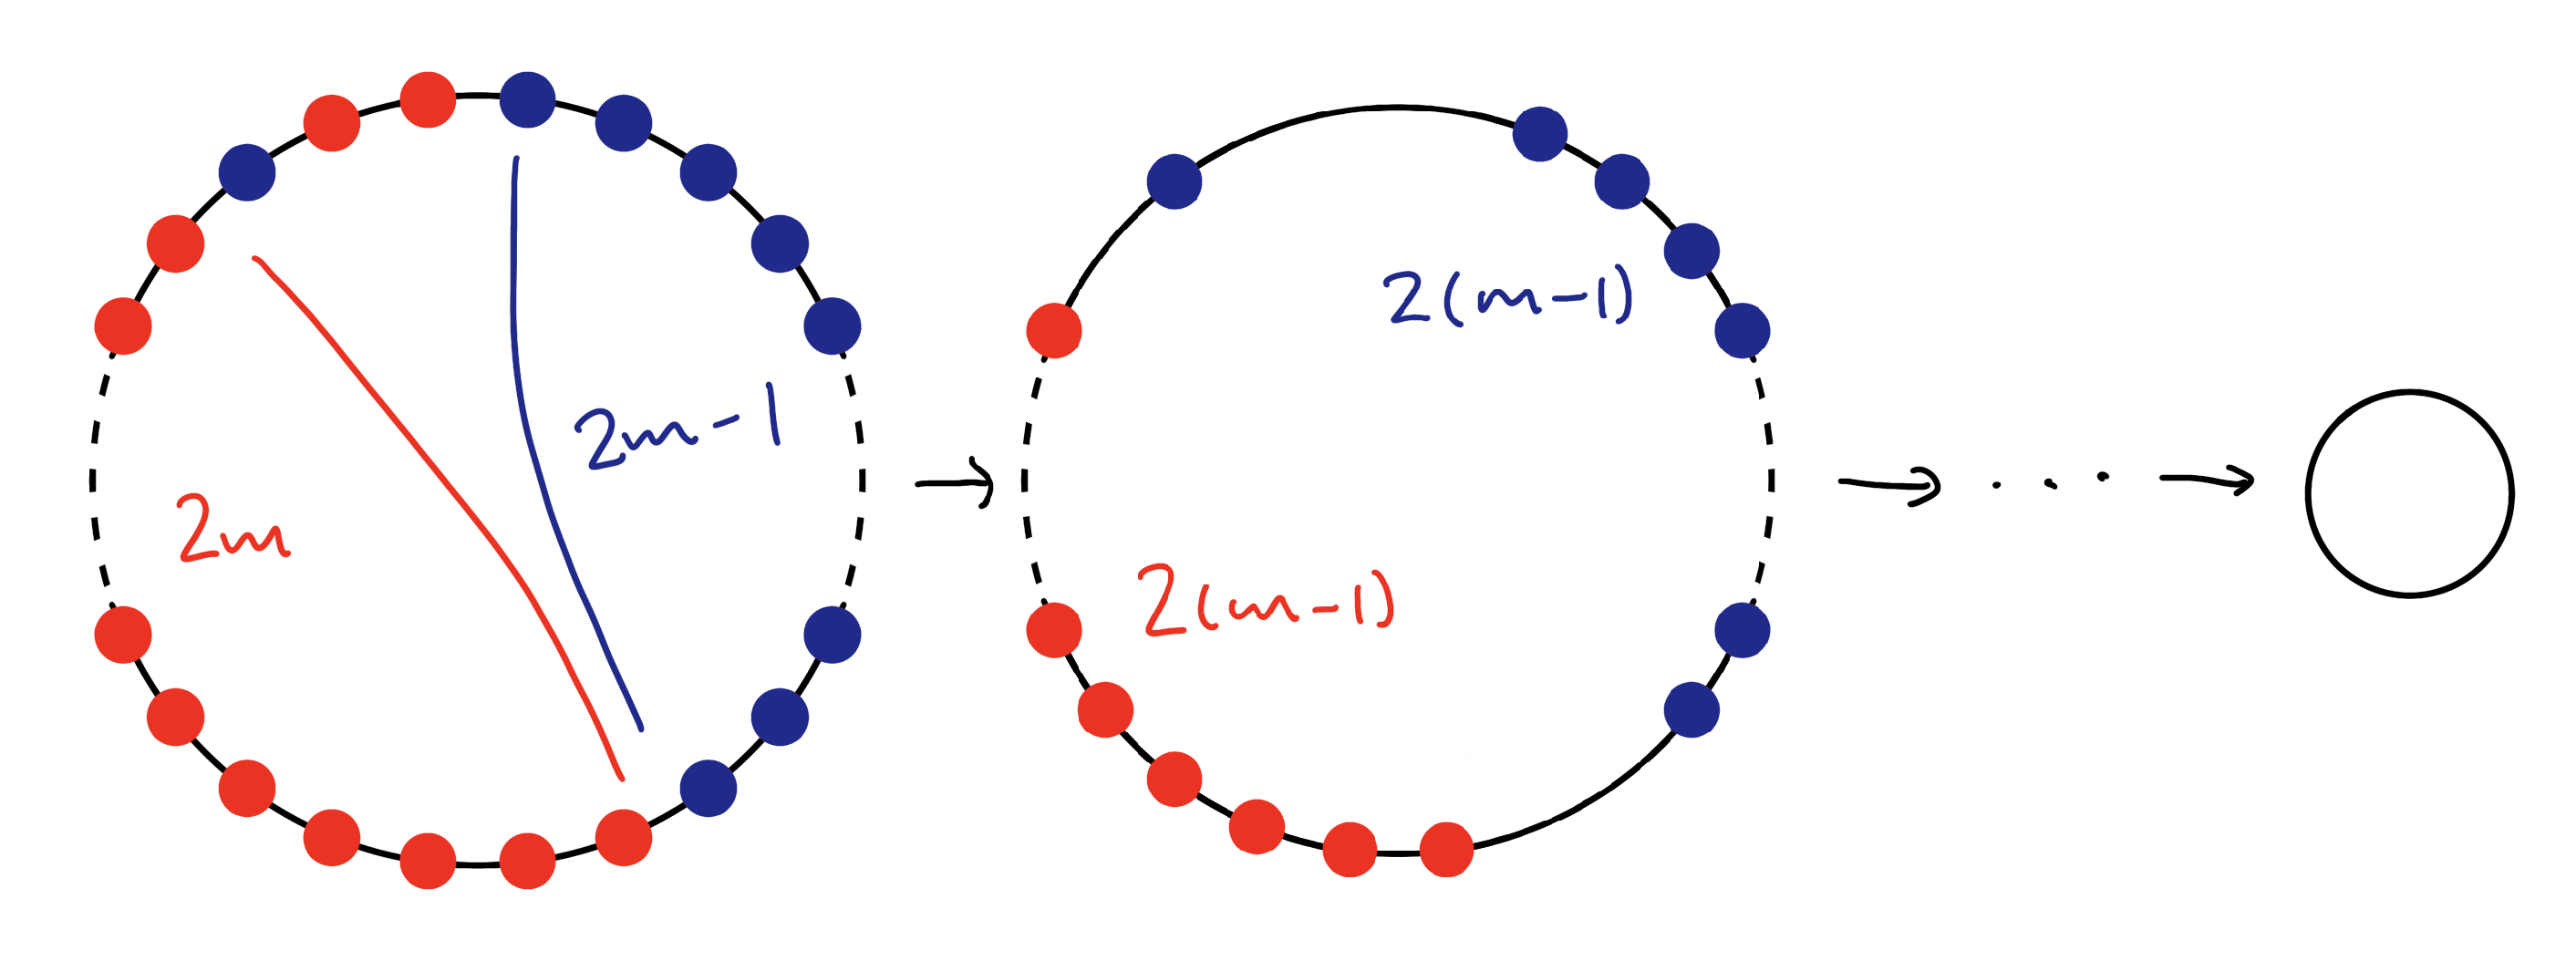
\includegraphics[width=11cm]{slow6.png}
    \vspace{-0.3cm}
\end{figure}
\end{document}